\section{Evaluation}


\subsection{Metrics}
We measure the algorithm performance using distance to the goal (in cm) at each step \ben{(lower is better)}. \ben{ \sout{The faster an algorithm reaches a certain distance the better.}} Note that the pixel size is around 1.6cm in our trajectory image encoding and 0.7cm in \ben{the} real world tracking image.



\subsection{Ablation Study in Simulation}

\textbf{Setup} We compare different variations of our method as well as some baseline methods to show the efficacy of our method in simulation. We randomly sampled 5 ropes for both interpolation and extrapolation part of the test set with respect to the training set. For each rope, we randomly sampled 25 goals that is guaranteed to be reachable. For each trial, iterative algorithms run for 16 steps. The distance to the goal (in cm) averaged for each step across all goals and ropes is reported in fig. \ref{fig:sim}.

\textbf{Benefit of Implicitly Capturing System Parameters}
One obvious approach to this task is to first identify key system parameters, and then compute the optimal action to the goal using the identified parameters. We give this baseline a head start by providing the true varying parameters: length and density. To ensure fairness, we assume 16 fixed system identification actions are executed (equal to the maximum amount of information known by our method), and the resulting 16 trajectories are provided as input. We train a ResNet-50 network using the 16 trajectory images to regress the rope parameters. Another 4-layer MLP neural network, that takes in the rope parameter and goal, is trained to regress the action using optimal actions computed by brute-force on the training dataset. As shown in orange, labeled as "sysid" in fig. \ref{fig:sim}, it averages 10.4 cm error for interpolation ropes and 24.8 cm error for extrapolation ropes, significantly under-performs our method. Even if we assume we know the test rope parameter perfectly, as shown in brown and labeled as "plan" in fig. \ref{fig:sim}, the performance improvement is marginal. \shuran{what is the conclusion??}

\textbf{benefit of residual formulation }
Single step, delta action, but 

\textbf{Effect of action representation.}
Instead of \ben{\sout{representing} providing} delta actions as input to the network, and sampl\ben{\sout{e}ing candidate} delta actions at test time, \ben{\sout{here we will let the} we instead use a} network to directly regress \ben{the} optimal delta action. We train a ResNet-50 network, taking the current trajectory image and the goal (represented as a one-hot image) to regress the delta action, trained using brute-force computed optimal action on the training set. This iterative algorithm is initialized using the same action as our algorithms, and it's step size multiplied with a tuned proportional gain. As shown in pink and labeled "action\_direction", this method yields 4.6cm and 9.8cm error in the final step on interpolation and extrapolation ropes respectively. \ben{Ben: I would explicitly remind readers of the implicit action performance here too. These numbers don't mean much without a comparison.}

\textbf{Benefit of Adaptive Action Sampling.}
Inspired by proportional control, we compute the \ben{\sout{sigma} variance} of the action sampling Gaussian distribution by multiplying the current distance to the goal with a constant gain. Without this feature, shown in grey and labeled "const\_sigma" in fig. \ref{fig:sim}, the algorithm has difficulty converging to the optimal action. \ben{Ben: Discuss why?}

\textbf{Heuristic Baseline.}
\ben{Ben: I wouldn't phrase it like this. I think something like "to provide context for the performance of our approach, we compare against a trivial heuristic strategy:" ...}
One might argue that our algorithm has learned a trivial strategy: decrease both the speed and amplitude of the action if the goal is in between the trajectory and the origin (i.e. inside the trajectory) and increase both if otherwise. As shown in green and labeled "heuristic" in fig. \ref{fig:sim}, this heuristic policy converges very slowly on extrapolation ropes and diverges on interpolation ropes. Note that the step size of this heuristic policy is also proportional to the error, and the gain has been tuned for the optimal result. \shuran{why it doesn't work}

\subsection{Real World Evaluation}
\textbf{Experiment Setup.}
To test our method's generalizability against the sim-to-real gap, we \ben{\sout{tested} evaluated} our method on 9 different real-world setups. We tested a thin cotton rope (13g/m) of 3 different lengths (75cm, 100cm, 125cm), a thick cotton rope (65g/m, 1m in length), a leather bullwhip (72g/m, 1m in length) and a piece of red cloth (1m in length). We modeled the simulation rope after the thin cotton rope, therefore other ropes \ben{\sout{should be considered} are significantly} out-of-distribution. In particular, the red cloth \ben{---} due to much larger surface area to density ratio \ben{---{} behaves very differently from a typical rope. }

\shuran{it is method not evaluation}
To obtain the rope tip trajectory as an input of our algorithm, we trained a tracking model based on DeeplLabV3+ with 400 hand labeled images. The tracking error on the validation set is 1.8 pixels, which translates to 1.3 cm for our setup. 

To speedup the data collection process, we terminate the algorithm once the error has reached 1.6 cm.


\textbf{Sim2Real Adaptation.}
The evaluation result has been summarized in Tab. \ref{tab:real_eval}. We compare against 2 baselines. NN: Optimal action (computed using brute force) for the nearest neighbor rope in terms of rope parameter. AVG: The action that minimizes the average distance to goal in the training set, regardless of rope parameter. Note that our method is initialized using this action. As shown in the Tab. \ref{tab:real_eval}, our method outperforms both baseline by a significant margin, and is very close to the tracking error. This result is particularly impressive for the red cloth. More details about of each steps of our algorithm has been shown in Fig. \ref{fig:real_detail}.
\shuran{point you want to make, iterative approach bridge the sim2real gap?}

\textbf{Online Adaptation.}
One advantage of using an interactive adjustment algorithm is the robustness against dynamic system changes. In this experiment, we first run the algorithm on the thin cotton rope (13g/m, 1m in length) for 6 steps. Just before step 7, we pause the robot and tie 3 knots that significantly changes the rope's length, density and mass distribution. As shown in Fig. \ref{fig:online_adaptation}, our algorithm quickly adjust\ben{ed} to the \ben{\sout{new} changed} system \ben{dynamics} and returned to the low error state. 


\begin{figure*}
    \centering
    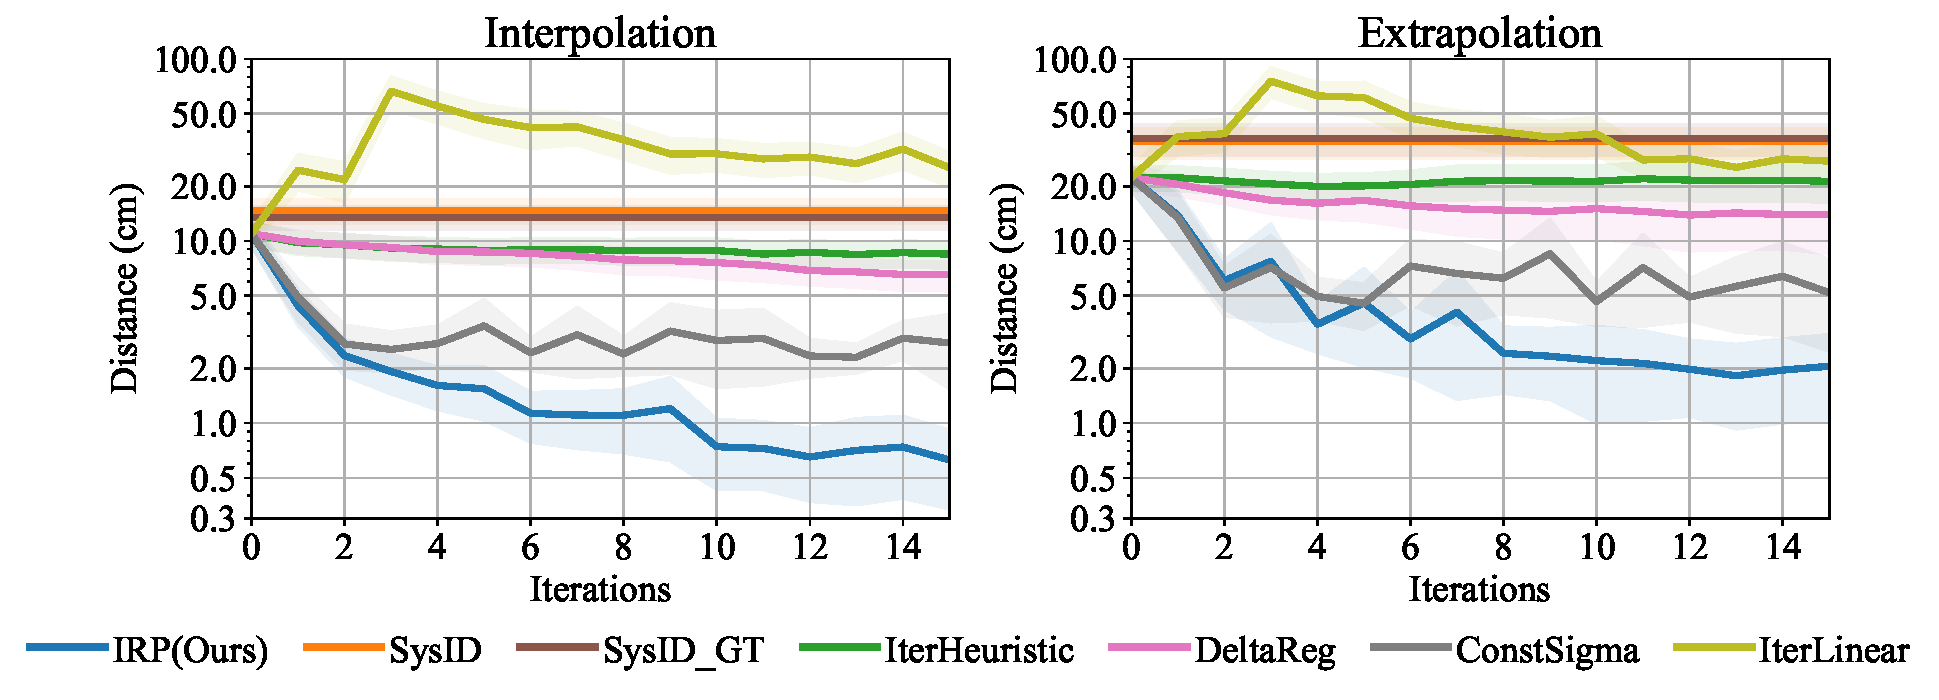
\includegraphics[width=0.66\linewidth]{figure/sim_plots.pdf} ~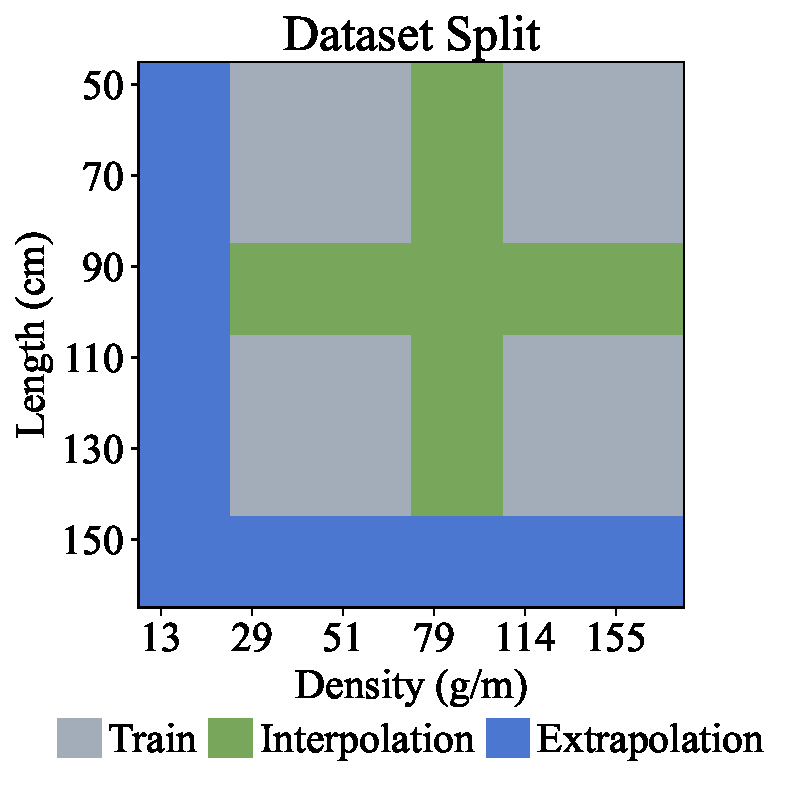
\includegraphics[width=0.3\linewidth]{figure/split_plot.pdf}
    \caption{\textbf{Simulation Evaluation.} Distance to goal in cm averaged across 5 ropes and 25 goals for each method, shown with 95\% confidence interval. Test rope parameters that are extrapolation with respect to training ropes (right) yield higher errors in general comparing to interpolation (left). The result of single-step methods (sysid, plan) are shown as lines for visualization.
    
    \textbf{Dataset Split.} \shuran{train. test - interpolation. test - extrapolation} \shuran{Same Y axis limit}
    The $12\times12$ grid of rope parameters used for simulation. In total, there are $64,31,49$ ropes in the training,validation and testing set respectively.}
    \label{fig:sim}
\end{figure*}

\begin{figure}
    \centering
    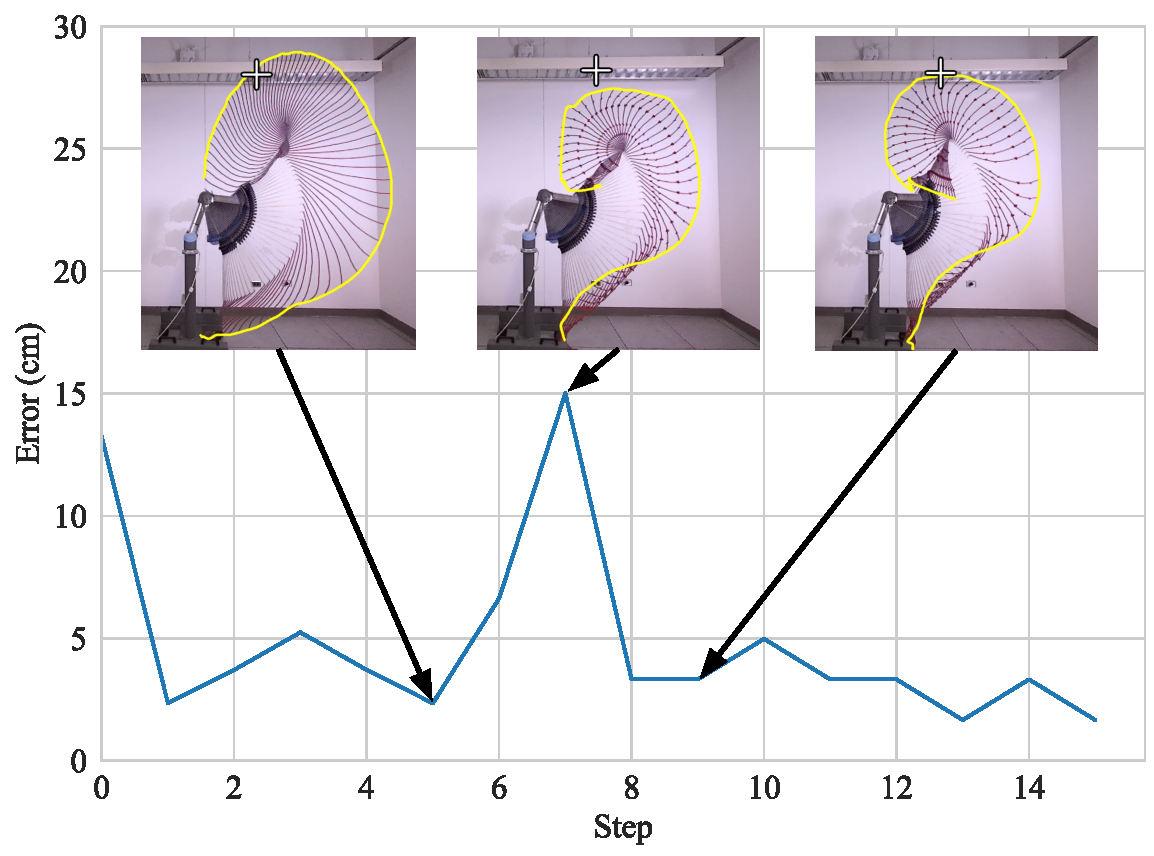
\includegraphics[width=\linewidth]{figure/interrupt_plot.pdf}
    \caption{\textbf{Online Adaptation.} Error plot of our algorithm tested on a thin cotton rope. Just before step 7, we paused the experiment and tied 3 knots on the rope that significantly changed the rope's length, density and mass distribution. Our algorithm quickly adapted to this change in the system afterwards.}
    \label{fig:online_adaptation}
    % https://docs.google.com/drawings/d/113vNeGlj8giXRdVfd47gkosV1PIefxu8HKGWcSKNlh8/edit?usp=sharing
\end{figure}


\begin{figure}
    \centering
     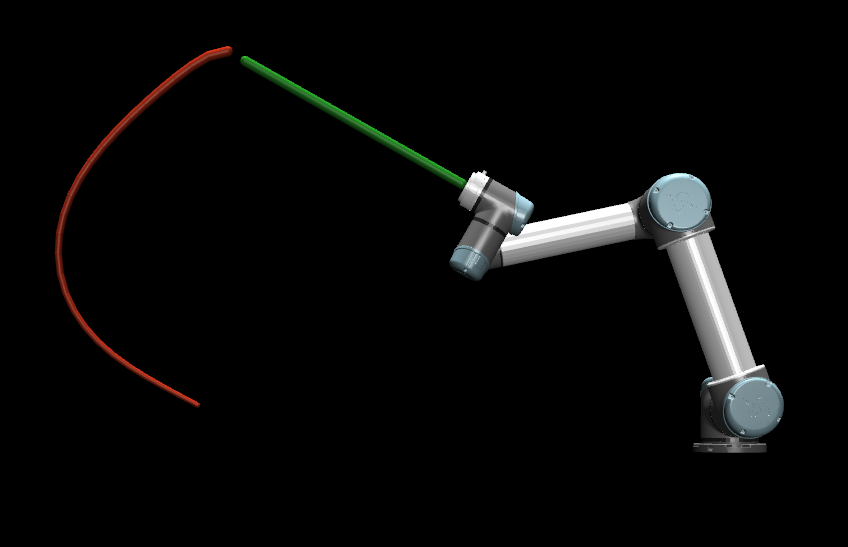
\includegraphics[width=\linewidth]{figure/mujoco_ur5.png}
    \caption{\textbf{MuJoCo simulation.} A UR5 robot swings a rope via an extension stick. The rope is modeled using 25 connected capsules.}
    \label{fig:mujoco}
\end{figure}


\begin{table}[]
    \begin{tabular}{lrrrr}
    \toprule
    {} &    NN &   AVG &  Ours Step3 &  Ours Step9 \\
    \midrule
    long\_stick\_thin\_red &  9.94 & 11.33 &        2.13 &        1.33 \\
    red\_cloth           & 26.72 & 30.43 &        7.00 &        0.99 \\
    short\_thin\_red      &  8.71 & 10.17 &        4.54 &        2.81 \\
    thick\_red           & 11.68 & 10.05 &        5.95 &        1.66 \\
    thin\_black          & 11.38 & 14.66 &        4.58 &        0.99 \\
    thin\_red            &  8.23 &  7.98 &        1.66 &        0.66 \\
    \bottomrule
    \end{tabular}
    % \begin{tabular}{lrrrrrr}
    % \toprule
    % {} &  long\_stick\_thin\_red &  red\_cloth &  short\_thin\_red &  thick\_red &  thin\_black &  thin\_red \\
    % \midrule
    % NN   &                 9.94 &      26.72 &            8.71 &      11.68 &       11.38 &      8.23 \\
    % AVG  &                11.33 &      30.43 &           10.17 &      10.05 &       14.66 &      7.98 \\
    % Ours &                 1.33 &       0.99 &            2.81 &       1.66 &        0.99 &      0.66 \\
    % \bottomrule
    % \end{tabular}
    \caption{\textbf{Real World Evaluation.} Distance to goal in cm in 6 real world ropes. red\_cloth and thin\_black are particularly out-of-distribution. NN: optimal action for most similar rope in the training set. AVG: action minimizes average error across all ropes in the training set. Ours: our method's error at step 3 and step 9.}
    \label{tab:real_eval}
\end{table}

\begin{figure*}
    \centering
    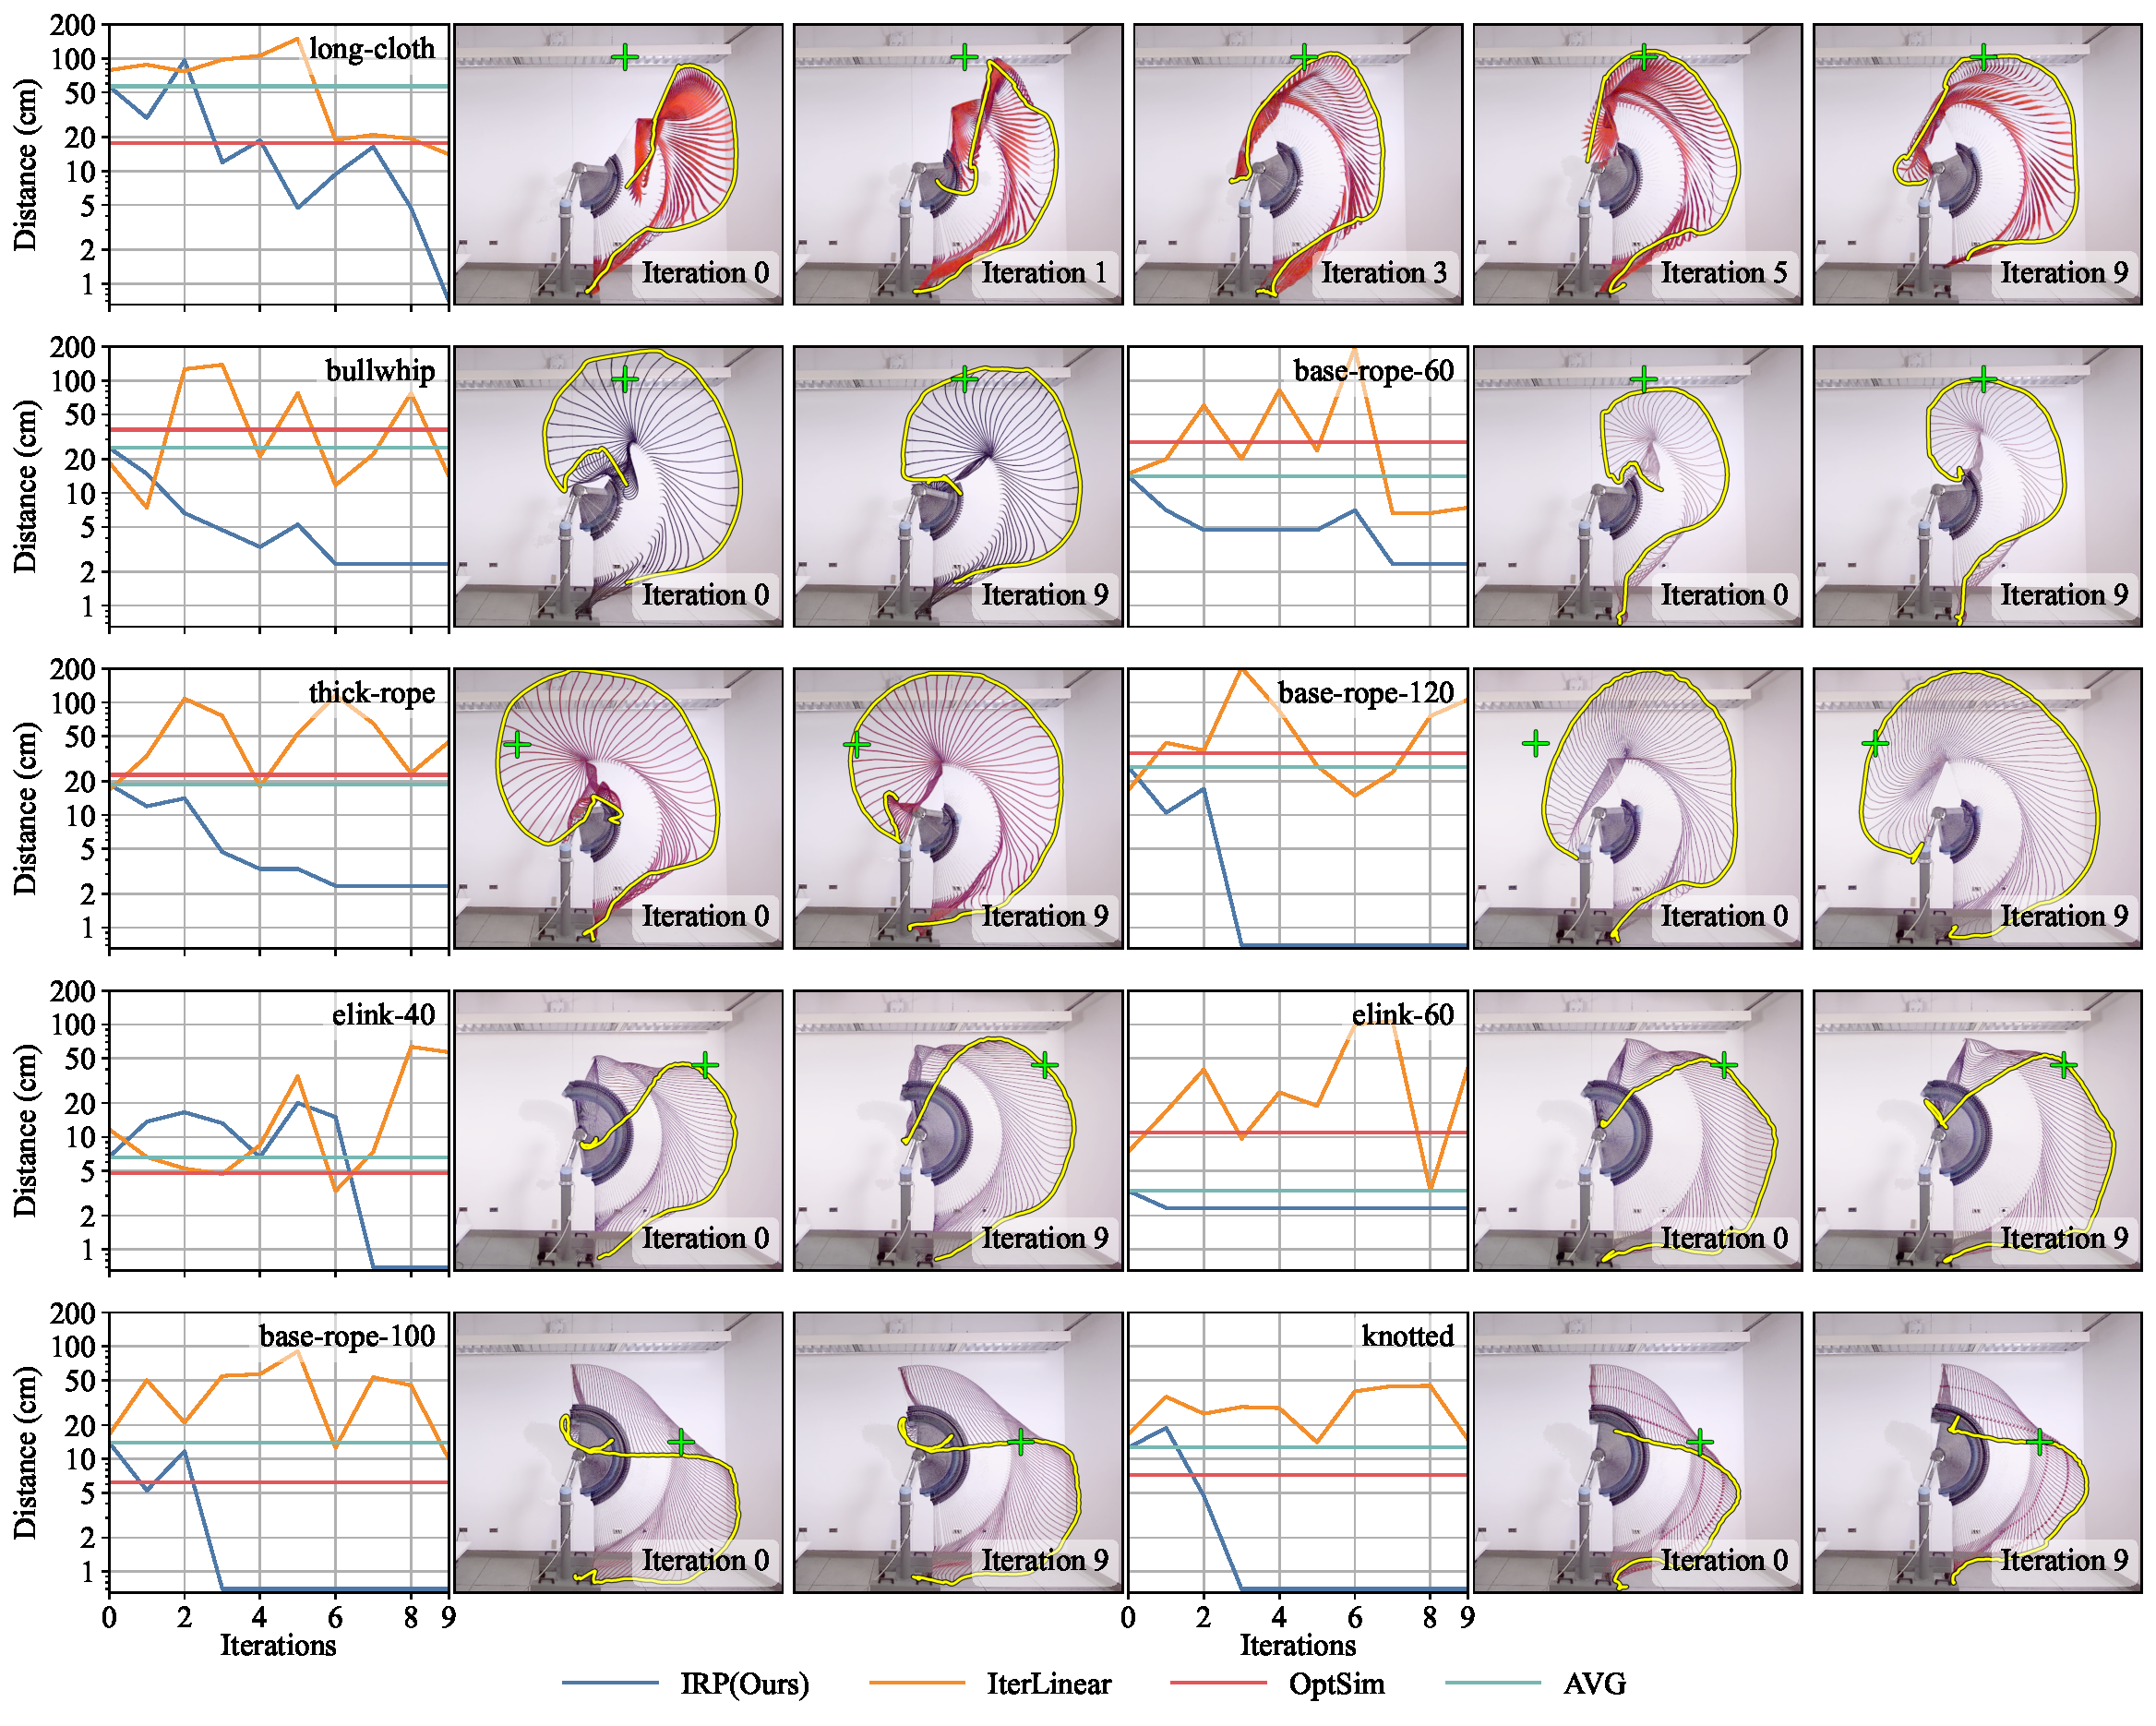
\includegraphics[width=\linewidth]{figure/real_vis_plots.pdf}
    \caption{\textbf{Results.} Left error plot for ours and baseline. Right, first, 5th, and last action trajectory for \names~and baselines. 
    \todo{make the line color consistent, make sure trajectory is visible, show rope and robot only for ours, other baseline only show trajectory}
    More results can be find in supp videos. \shuran{all the images has a strange white balance} }
    %https://docs.google.com/drawings/d/1oiWSkWwh9zzMQ_cAMQME6a0cPVZw53zplIQvz1UpmLs/edit?usp=sharing
    \label{fig:real_detail}
\end{figure*}


\section{Conclusion} 
\label{sec:conclusion}

The conclusion goes here. \ben{Ben: It might be helpful to put a few bullets here before too much more gets added to the main document. What's the big takeaway here, why is this strategy effective
and how would you what are the important take-aways?}